\section{OxRAM Device Physics}
\label{sec:bg-oxram}

Oxide-based ReRAM (OxRAM) is the most commercially mature class of
resistive memory. An OxRAM device consists of a metal oxide switching
layer sandwiched between two metal electrodes, forming a
metal-insulator-metal (MIM) stack~\cite{wong2012metal,chen2020reram}.
The switching layer is typically constructed from a transition metal
oxide such as HfO$_2$ or Ta$_2$O$_5$, both of which are high-$\kappa$
dielectrics already present in standard CMOS process
flows~\cite{wong2012metal, chen2020reram}. This process compatibility
enables OxRAM devices to be integrated at the back-end-of-line (BEOL)
alongside the upper metal layers of a semiconductor device, without
modification to the front-end transistor process. OxRAM bitcells are
formed at the intersections of wordlines (WLs) and bitlines (BLs) in a
crossbar array, with an access transistor providing cell
isolation~\cite{wong2012metal}.

\begin{figure}[t!]
	\centering
	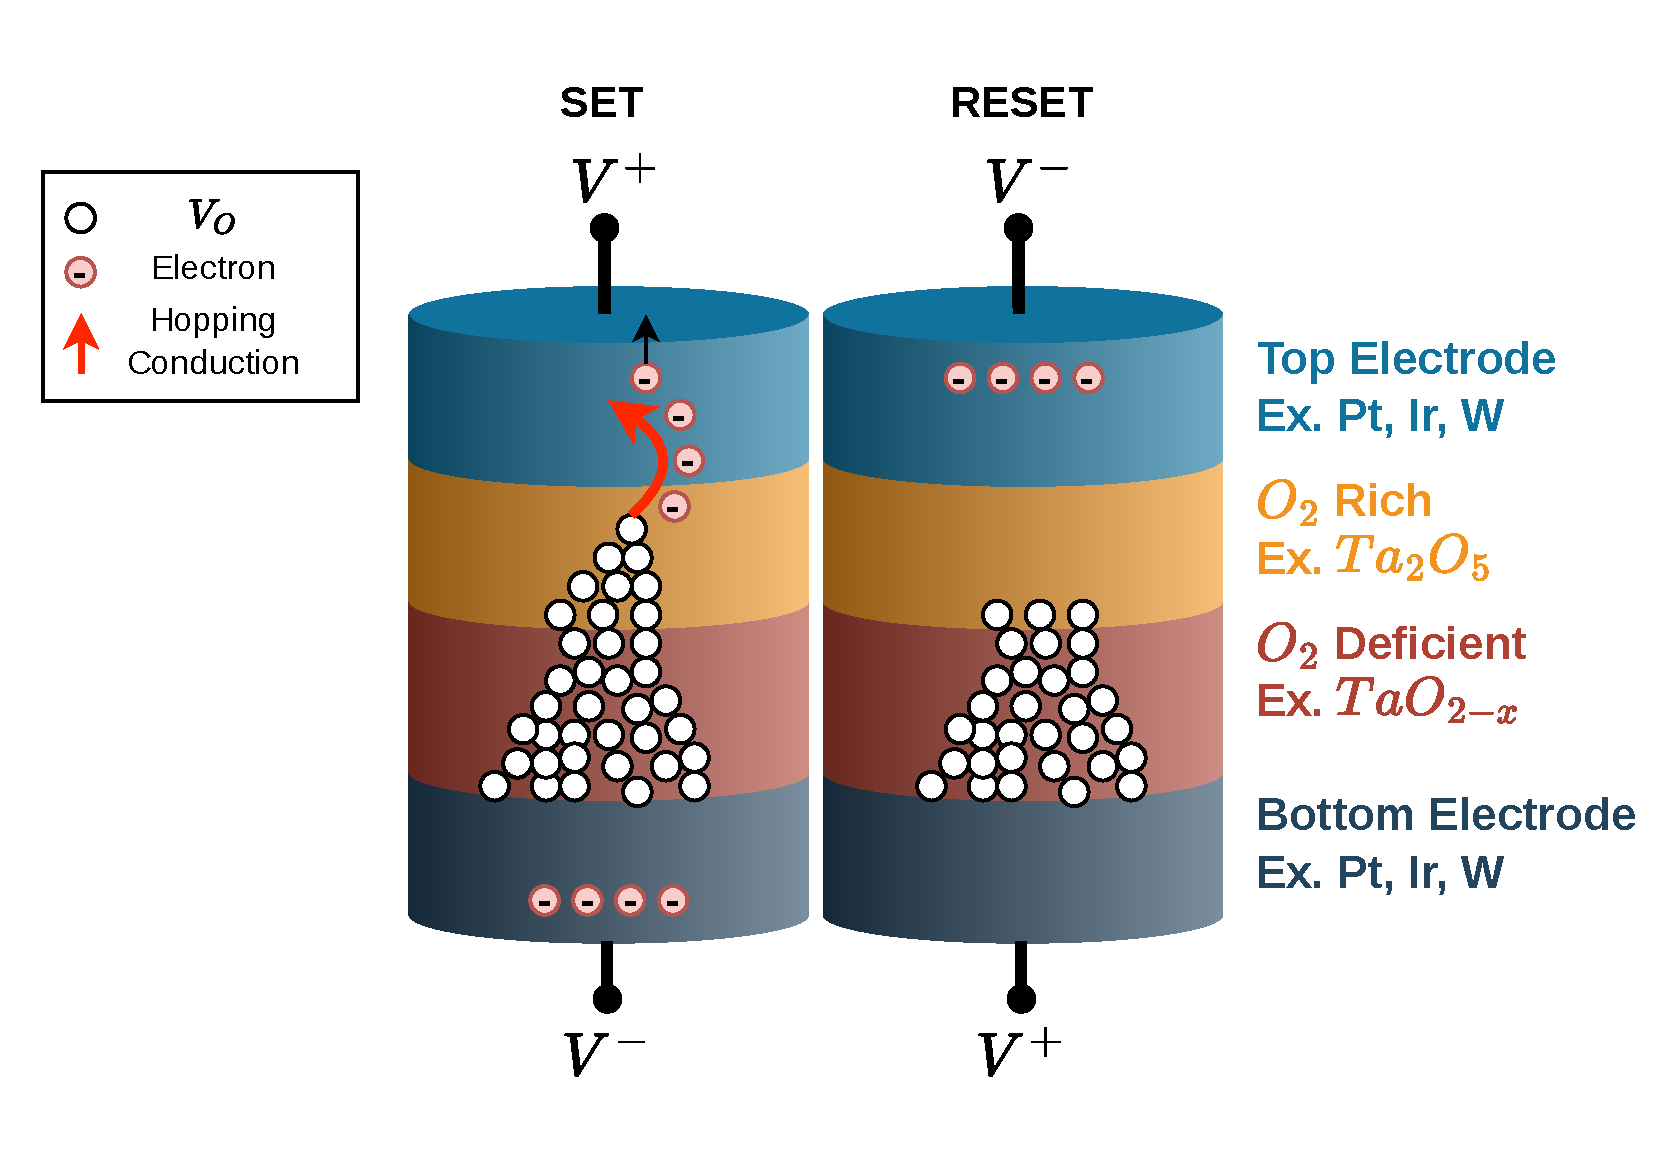
\includegraphics[width=0.9\linewidth]{img/ReRAMDiagram.pdf}
	\caption{Diagram of bipolar OxRAM SET, and RESET physics. The top and bottom electrodes can be either inert (e.g. Pt) or reactive (e.g. W) materials. A switching bi-layer is used to control filament growth. The $O_2$ deficient region acts as a vacancy reservoir. The $O_2$ rich region attracts these vacancies under an electric field. During the set operation, the device is set into its LRS, and hopping conduction under the programming voltage can cause a spike in current, which needs to be limited to avoid damage to the cell.}
	\label{fig:oxram-prog}
\end{figure}

OxRAM devices typically operate in a bipolar switching regime, in which
the polarity of the applied voltage determines whether the device
transitions to a low-resistance state (LRS) or a high-resistance state
(HRS)~\cite{wong2012metal, chen2020reram}. A SET operation applies a
positive voltage across the device, driving oxygen ions out of the
switching layer and leaving behind a chain of oxygen vacancies that form
a conductive filament (CF) bridging the two
electrodes~\cite{wei2008highly, yu2012switching}. The completed filament
is the LRS. A RESET operation applies a voltage of the opposite
polarity, which drives oxygen ions back into the filament region,
rupturing the CF and returning the device to the
HRS~\cite{yu2012switching}. The LRS and HRS correspond to stored logical
values and are distinguished by their resistance ratio
$R_\text{OFF}/R_\text{ON}$, which is typically in the range of
$10$-$10^3$ for commercial OxRAM devices~\cite{chen2020reram}.

The switching dynamics of OxRAM devices are controlled by the local
electric field, the thermal profile of the device, and the stochastic
availability of oxygen vacancies at the filament
tip~\cite{yu2012switching}. SET and RESET operations are asymmetric: SET
requires nucleation and growth of a new filament segment and is
therefore more sensitive to the initial CF state, while RESET requires
rupture of an existing structure~\cite{yu2012switching, wei2008highly}.
This asymmetry produces data-dependent differences in switching dynamics
that are observable through write latency measurements. The stochastic
nature of oxygen vacancy migration means that the number of programming
pulses required to complete a transition varies from cycle to cycle,
even under identical initial conditions~\cite{fantini2013intrinsic,
	ambrogio2013understanding}. This cycle-to-cycle variability is the
fundamental physical source of the timing entropy and side-channel
signals studied in this dissertation.